\section{Разработка модифицированного алгоритма SCC}

На~базе описанного метода был реализован модифицированный частичный алгоритм, использующий рекурсию.
Алгоритм получил название~\emph{SCC}
(\emph{Strong Cyclicity \newline Checking}).
В отличие от~предыдущего алгоритма, который выбирает для~продолжения лишь один элемент матрицы,
модифицированный алгоритм будет перебирать все возможные элементы для~продолжения.

Вход алгоритма:
\begin{itemize}
    \item
        квадратная матрица~$A$ размера $m \times m$ с~полиномиальными коэффициентами;
    \item
        циклический вектор~$v$;
    \item
        максимальная глубина рекурсии~$depth$.
\end{itemize}

Выход алгоритма "--- один из~следующих ответов:
\begin{itemize}
    \item
        <<не сильно циклический>> + продолжение, опровергающее сильную цикличность;
    \item
        <<сильно циклический>>;
    \item
        <<неизвестно>>.
\end{itemize}

Шаги алгоритма:
\begin{enumerate}
    \item
        Если $depth = 0$, вернуть ответ~<<неизвестно>>.
    \item
        Положить $solutions = $ пустой список.
        Этот список будет содержать тройки вида~$(i, j, sol)$,
        где $i, j$ "--- номера элементов матрицы, $sol$ "--- некоторый числовой коэффициент,
        которым следует продолжить данный элемент.
    \item
        Перебираем все элементы матрицы с~номерами~$(i, j)$ в некотором порядке (например, сначала по~строкам, затем по~столбцам):
        \begin{enumerate}
            \item
                Копируем матрицу~$A$ в матрицу~$B$: $B = Copy(A)$;
            \item
                Определяем степень текущего элемента~$B_{ij}$ как многочлена от~$x$:
                $t = degree(B_{ij})$;
            \item
                Продолжаем текущий элемент матрицы слагаемым с~символьным коэффициентом~$c$:
                $B_{ij} += cx^{t + 1}$;
            \item
                Находим $det(c, x)$ "--- определитель матрицы \diffMatrix[B] как многочлен от~$x$,
                коэффициенты которого "--- многочлены от~$c$;
            \item
                Находим все ненулевые значения~$c$, зануляющие~$\tc(det(c, x))$;
                \begin{enumerate}
                    \item
                        Если какое-то значение~$c$ зануляет весь~$det(c, x)$,
                        то мы нашли опровергающее продолжение.
                        Подставляем в~матрицу~$B$ данное числовое значение вместо символа~$c$,
                        возвращаем ответ~<<не сильно циклический>> и матрицу~$B$ в~качестве опровергающего продолжения.
                \end{enumerate}
            \item
                Добавляем все найденные значения~$c$ в~список $solutions$ как тройки~$(i, j, sol)$.
        \end{enumerate}
    \item
        Перебираем все тройки $(i, j, sol)$ из~списка $solutions$:
        \begin{enumerate}
            \item
                Копируем матрицу~$A$ в матрицу~$B$: $B = Copy(A)$;
            \item
                Продолжаем элемент матрицы $(i, j)$ слагаемым с~числовым коэффициентом $sol$:
                $B_{ij} += sol \cdot x^{degree + 1}$;
            \item
                \textbf{Рекурсивно} применяем данный алгоритм
                к~матрице~$B$, вектору~$v$ и глубине рекурсии~$depth - 1$;
            \item
                Если был получен ответ~<<не сильно циклический>> + продолжение, вернуть данный ответ и продолжение.
        \end{enumerate}
    \item
        Если на предыдущем шаге хотя бы в одном случае был получен ответ~<<неизвестно>>, вернуть ответ~<<неизвестно>>.
    \item
        Вернуть ответ~<<сильно циклический>>.
\end{enumerate}

Данный алгоритм всегда завершается благодаря ограниченной глубине рекурсии,
но он все~еще не~всегда может дать содержательный ответ.
Однако, такие ситуации должны быть более редкими, поскольку перебираются все элементы матрицы для~продолжения,
и в~случае захода в~тупик будет производиться возврат и выбор следующего варианта.

Возможный ход работы алгоритма представлен на рис. 6.1:

\begin{center}
    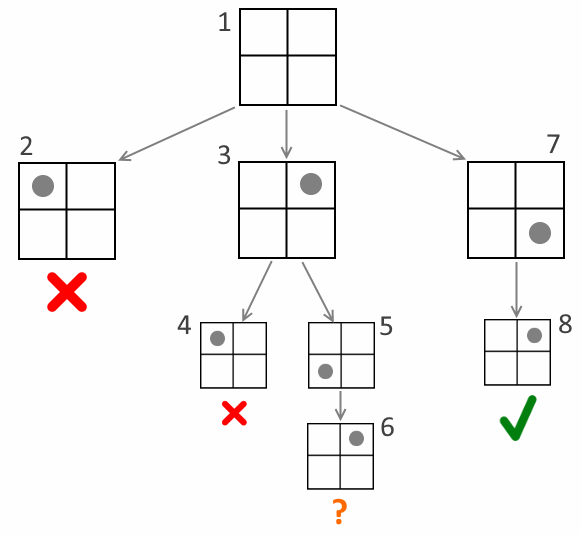
\includegraphics[scale=0.6]{pictures/recursion.png}

    \small
    Рис. 6.1. Ход работы алгоритма
\end{center}

Пусть на вход алгоритму поступили матрица размера~$2 \times 2$ и некоторый вектор~$v$.
\begin{enumerate}
    \item
        Изначально мы находимся в~ситуации~1.
        В~этой ситуации у нас есть три варианта построить одноэлементное продолжение:
        можно продолжить левый верхний элемент матрицы (это соответствует ситуации~2),
        правый верхний~(3) и правый нижний~(7).
        По~очереди рекурсивно вызываем процедуру от~указанных вариантов.
    \item
        Попали в~ситуацию~2. Отсюда невозможно продолжить построение опровергающего продолжения,
        возвращаем на предыдущий уровень~(1) ответ~<<сильно циклический>> и рассматриваем следующий вариант.
    \item
        Попали в~ситуацию~3. Здесь есть два способа построить одноэлементное продолжение,
        которые приведут нас в~ситуации~4~и~5.
        По~очереди рекурсивно вызываем процедуру от~указанных вариантов.
    \item
        Попали в~ситуацию~4. Отсюда невозможно продолжить построение опровергающего продолжения,
        возвращаемся на предыдущий уровень~(3) с~ответом~<<сильно циклический>> и рассматриваем следующий вариант.
    \item
        Попали в~ситуацию~5. Здесь есть единственный вариант для~построения продолжения,
        отсюда мы попадем в~ситуацию~6.
    \item
        Попали в~ситуацию~6. Здесь оказывается, что была достигнута максимально допустимая глубина рекурсии.
        Возвращаем на~предыдущий уровень~(5) ответ~<<неизвестно>>,
        оттуда, в~свою~очередь, также вернется ответ~<<неизвестно>> на~предыдущий уровень~(3),
        а оттуда, аналогично, этот ответ попадет на~самый верхний уровень~(1).
    \item
        Попали в~ситуацию~7. Здесь есть единственный вариант для~построения продолжения,
        отсюда мы попадем в~ситуацию~8.
    \item
        Попали в~ситуацию~8. Здесь есть единственный вариант для~построения продолжения,
        причем это продолжение является опровергающим (определитель равен нулю).
        Возвращаем ответ~<<не сильно циклический>> и построенное продолжение,
        этот ответ и будет финальным результатом алгоритма.
\end{enumerate}
